\chapter{EPICS Overview}

\section{What is EPICS?}

\index{EPICS}
The Experimental Physics and Industrial Control System (EPICS) consists of a set of software components and tools that
Application Developers can use to create control systems. The basic components are:

\begin{itemize}
\item \textbf{OPI}: \index{OPI}Operator Interface. This is a workstation which can run various EPICS tools.

\item \textbf{IOC}: \index{IOC}Input/Output Controller. Any platform that can support EPICS run time databases together with the other 
software components described in the manual. One example is a workstation. Another example is a VME/VXI 
based system using vxWorks or RTEMS as the realtime operating system.

\item \textbf{LAN}: \index{LAN}Local Area Network. This is the communication network which allows the IOCs and OPIs to communicate. 
EPICS provides a software component, \index{Channel Access}Channel Access, which provides network transparent communication 
between a Channel Access client and an arbitrary number of Channel Access servers.
\end{itemize}

A control system implemented via EPICS has the following physical structure.

\begin{center}
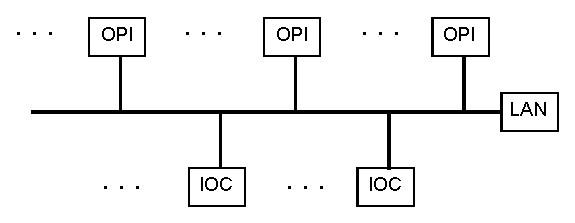
\includegraphics{overview_1}
\end{center}

The rest of this chapter gives a brief description of EPICS:

\begin{itemize}
\item \textbf{Basic Attributes}: A few basic attributes of EPICS.
\item \textbf{Platforms}: The vendor supplied Hardware and Software platforms EPICS supports.
\item \textbf{IOC Software}: EPICS supplied IOC software components.
\item \textbf{Channel Access}:  EPICS software that supports network independent access to IOC databases.
\item \textbf{OPI Tools}: EPICS supplied OPI based tools.
\item \textbf{EPICS Core}: A list of the EPICS core software, i.e. the software components without which EPICS will not work.
\end{itemize}

\section{Basic Attributes}

\index{EPICS!Basic Attributes}
The basic attributes of EPICS are:

\begin{itemize}

\item \textbf{Tool Based}: EPICS provides a number of tools for creating a control system. This minimizes the need for custom 
coding and helps ensure uniform operator interfaces.

\item \textbf{Distributed}: An arbitrary number of IOCs and OPIs can be supported. As long as the network is not saturated, no 
single bottle neck is present. A distributed system scales nicely. If a single IOC becomes saturated, its functions can 
be spread over several IOCs. Rather than running all applications on a single host, the applications can be spread 
over many OPIs.

\item \textbf{Event Driven}: The EPICS software components are all designed to be event driven to the maximum extent 
possible. For example, rather than having to poll IOCs for changes, a Channel Access client can request that it be 
notified when a change occurs. This design leads to efficient use of resources, as well as, quick response times.

\item \textbf{High Performance}: A SPARC based workstation can handle several thousand screen updates a second with each 
update resulting from a Channel Access event. A 68040 IOC can process more than 6,000 records per second, 
including generation of Channel Access events. 

\end{itemize}

\section{IOC Software Components}

\index{Input/Output Controller!Software Components}

An IOC contains the following EPICS supplied software components.

\begin{center}
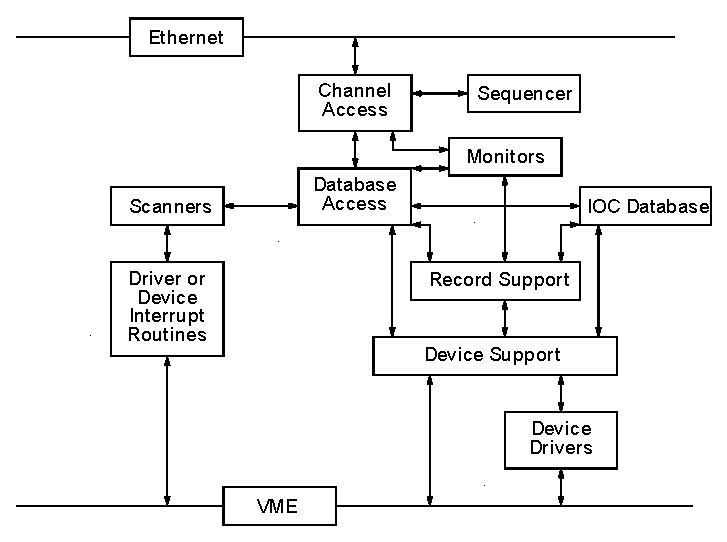
\includegraphics{overview_6}
\end{center}

\begin{itemize}
\item \textbf{IOC Database}: The memory resident database plus associated data structures.

\item \textbf{Database Access}:  Database access routines. With the exception of record and device support, all access to the 
database is via the database access routines.

\item \textbf{Scanners}:  The mechanism for deciding when records should be processed.

\item \textbf{Record Support}:  Each record type has an associated set of record support routines.

\item \textbf{Device Support}: Each record type can have one or more sets of device support routines.

\item \textbf{Device Drivers}:  Device drivers access external devices. A driver may have an associated driver interrupt routine.

\item \textbf{Channel Access}:  The interface between the external world and the IOC. It provides a network independent 
interface to database access.

\item \textbf{Monitors}:  Database monitors are invoked when database field values change.

\item \textbf{Sequencer}:  A finite state machine.
\end{itemize}

Let's briefly describe the major components of the IOC and how they interact.

\subsection{IOC Database}

The heart of each IOC is a memory resident database together with various memory resident structures describing the 
contents of the database. EPICS supports a large and extensible set of record types, e.g. \verb|ai| (Analog Input), \verb|ao| (Analog 
Output), etc.

Each record type has a fixed set of fields. Some fields are common to all record types and others are specific to particular 
record types. Every record has a record name and every field has a field name. The first field of every database record 
holds the record name, which must be unique across all IOCs that are attached to the same TCP/IP subnet.

Data structures are provided so that the database can be accessed efficiently. Most software components, because they 
access the database via database access routines, do not need to be aware of these structures.

\subsection{Database Access}

With the exception of record and device support, all access to the database is via the channel or database access routines. 
See Chapter 15, ``Runtime Database Access" on page213 FIXPAGEREF for details.

\subsection{Database Scanning}

Database scanning is the mechanism for deciding when to process a record. Five types of scanning are possible: Periodic, 
Event, I/O Event, Passive and Scan Once.

\begin{itemize}
\item \textbf{Periodic}:  A request can be made to process a record periodically. A number of time intervals are supported.

\item \textbf{Event}:  Event scanning is based on the posting of an event by any IOC software component. The actual subroutine 
call is: \\
\verb|post_event(event_num)|\index{post\_event}
\item \textbf{I/O Event}:  The I/O event scanning system processes records based on external interrupts. An IOC device driver 
interrupt routine must be available to accept the external interrupts.

\item \textbf{Passive}:  Passive records are processed as a result of linked records being processed or as a result of external 
changes such as Channel Access puts.

\item \textbf{Scan Once}: In order to provide for caching puts, The scanning system provides a routine \verb|scanOnce| which 
arranges for a record to be processed one time.
\end{itemize}

\subsection{Record Support, Device Support and Device Drivers}

Database access needs no record-type specific knowledge, because each record-type has its associated record support 
module. Therefore, database access can support any number and type of records. Similarly, record support contains no 
device specific knowledge, giving each record type the ability to have any number of independent device support 
modules. If the method of accessing the piece of hardware is more complicated than what can be handled by device 
support, then a device driver can be developed. 

Record types \emph{not} associated with hardware do not have device support or device drivers.

The IOC software is designed so that the database access layer knows nothing about the record support layer other than 
how to call it. The record support layer in turn knows nothing about its device support layer other than how to call it. 
Similarly the only thing a device support layer knows about its associated driver is how to call it. This design allows a 
particular installation and even a particular IOC within an installation to choose a unique set of record types, device types, 
and drivers. The remainder of the IOC system software is unaffected.

Because an Application Developer can develop record support, device support, and device drivers, these topics are 
discussed in greater detail in later chapters.

Every record support module must provide a record processing routine to be called by the database scanners. Record 
processing consists of some combination of the following functions (particular records types may not need all functions):

\begin{itemize}
\item \textbf{Input}:  Read inputs. Inputs can be obtained, via device support routines, from hardware, from other database 
records via database links, or from other IOCs via Channel Access links.

\item \textbf{Conversion}:  Conversion of raw input to engineering units or engineering units to raw output values.

\item \textbf{Output}:  Write outputs. Output can be directed, via device support routines, to hardware, to other database records 
via database links, or to other IOCs via Channel Access links.

\item \textbf{Raise Alarms}:  Check for and raise alarms.

\item \textbf{Monitor}:  Trigger monitors related to Channel Access callbacks.

\item \textbf{Link}:  Trigger processing of linked records.
\end{itemize}

\subsection{Channel Access}

Channel Access is discussed in the next section.

\subsection{Database Monitors}

Database monitors  provide a callback mechanism for database value changes. This allows the caller to be notified when 
database values change without constantly polling the database. A mask can be set to specify value changes, alarm  
changes, and/or archival changes. 

At the present time only Channel Access uses database monitors. No other software should use the database monitors.  
The monitor routines will not be described because they are of interest only to Channel Access.

\section{Channel Access}

Channel Access provides network transparent access to IOC databases. It is based on a client/ server model. Each IOC 
provides a Channel Access server which is willing to establish communication with an arbitrary number of clients. 
Channel Access client services are available on both OPIs and IOCs. A client can communicate with an arbitrary number 
of servers.

\subsection{Client Services}

The basic Channel Access client services are:

\begin{itemize}
\item \textbf{Search}:  Locate the IOCs containing selected process variables and establish communication with each one.

\item \textbf{Get}:  Get value plus additional optional information for a selected set of process variables.

\item \textbf{Put}:  Change the values of selected process variables.

\item \textbf{Add Event}: Add a change of state callback. This is a request to have the server send information only when the 
associated process variable changes state. Any combination of the following state changes can be requested: 
change of value, change of alarm status and/or severity, and change of archival value. Many record types provide 
hysteresis factors for value changes.
\end{itemize}

In addition to requesting process variable values, any combination of the following additional information may be 
requested:

\begin{itemize}
\item \textbf{Status}:  Alarm status and severity.

\item \textbf{Units}:  Engineering units for this process variable.

\item \textbf{Precision}:  Precision with which to display floating point numbers.

\item \textbf{Time}:  Time when the record was last processed.

\item \textbf{Enumerated}:  A set of ASCII strings defining the meaning of enumerated values.

\item \textbf{Graphics}:  High and low limits for producing graphs.

\item \textbf{Control}:  High and low control limits.

\item \textbf{Alarm}:  The alarm \verb|HIHI|, \verb|HIGH|, \verb|LOW|, and \verb|LOLO| values for the process variable.
\end{itemize}

It should be noted that Channel Access does not provide access to database records as records. This is a deliberate design 
decision. This allows new record types to be added without impacting any software that accesses the database via Channel 
Access, and it allows a Channel Access client to communicate with multiple IOCs having differing sets of record types.

\subsection{Search Server}

Channel Access provides an IOC resident server which waits for Channel Access search messages. These are generated 
when a Channel Access client (for example when an Operator Interface task starts) searches for the IOCs containing 
process variables the client uses. This server accepts all search messages, checks to see if any of the process variables are 
located in this IOC, and, if any are found, replies to the sender with and ``I have it" message.

\subsection{Connection Request Server}

Once the process variables have been located, the Channel Access client issues connection requests for each IOC 
containing process variables the client uses. The connection request server, in the IOC, accepts the request and establishes 
a connection to the client. Each connection is managed by two separate tasks: \verb|ca_get| and \verb|ca_put|. The \verb|ca_get| and 
\verb|ca_put| requests map to \verb|dbGetField| and \verb|dbPutField| database access requests. \verb|ca_add_event| requests result in 
database monitors being established. Database access and/or record support routines trigger the monitors via a call to 
\verb|db_post_event|.

\subsection{Connection Management}

Each IOC  provides a connection management service. When a Channel Access server fails (e.g. its IOC crashes) the 
client is notified and when a client fails (e.g. its task crashes) the server is notified. When a client fails, the server breaks 
the connection. When a server crashes, the client automatically re-establishes communication when the server restarts. 


\section{OPI Tools}

EPICS provides a number of OPI based tools. These can be divided into two groups based on whether or not they use 
Channel Access. Channel Access tools are real time tools, i.e. they are used to monitor and control IOCs.

\subsection{Examples of Channel Access Tools}

A large number of Channel Access tools have been developed. The following are some representative examples.

\begin{itemize}
\item \textbf{CSS}: Control System Studio, an Eclipse RCP application with many available plug-ins.

\item \textbf{EDM}: Extensible Display Manager.

\item \textbf{MEDM}: Motif Editor and Display Manager.

\item \textbf{StripTool}: A general-purpose stripchart program.

\item \textbf{ALH}: Alarm Handler. General purpose alarm handler driven by an alarm configuration file.

\item \textbf{Sequencer}:  Runs in an IOC and emulates a finite state machine.

\item \textbf{Probe}: Allows the user to monitor and/or change a single process variable specified at run time.
\end{itemize}

\subsection{Examples of other Tools}

\begin{itemize}
\item \textbf{VDCT}: A Java based database configuration tool which is quickly becoming the recommended database 
configuration tool.

\item \textbf{SNC}:  State Notation Compiler. It generates a C program that represents the states for the IOC Sequencer tool.
\end{itemize}

\section{EPICS Core Software}

EPICS consists of a set of core software and a set of optional components. The core software, i.e. the components of 
EPICS without which EPICS would not function, are:

\begin{itemize}
\item Channel Access - Client and Server software

\item IOC Database

\item Scanners

\item Monitors

\item Database Definition Tools

\item Source/Release
\end{itemize}

All other software components are optional. Of course, most applications will need equivalent functionality to
MEDM (or EDD/DM). Likewise an application developer would not start from scratch developing record and device 
support. Most OPI tools do not, however, have to be used. Likewise any given record support module, device support 
module, or driver could be deleted from a particular IOC and EPICS will still function.

